% TerraScope Crop Health Monitor -- IEEE conference paper (IEEEtran).
% Compile: pdflatex terrascope-ieee && bibtex terrascope-ieee && pdflatex terrascope-ieee && pdflatex terrascope-ieee
\documentclass[conference]{IEEEtran}
\IEEEoverridecommandlockouts

\usepackage{cite}
\usepackage{amsmath,amssymb,amsfonts}
\usepackage{graphicx}
\usepackage{textcomp}
\usepackage{xcolor}
\usepackage{booktabs}
\usepackage{multirow}
\usepackage{algorithm}
\usepackage{algpseudocode}
\usepackage{tikz}
\usetikzlibrary{positioning,arrows.meta,fit}
\usepackage{url}
\usepackage[hidelinks]{hyperref}

\graphicspath{{figures/}}
\newcommand{\NDVI}{\mathrm{NDVI}}

\begin{document}

\title{TerraScope: An Evidence-First, Provenance-Aware Platform for Field-Level Crop Health Monitoring with Sentinel-2 Imagery}

% TODO: replace with the actual author list, affiliations and e-mail addresses.
\author{
\IEEEauthorblockN{First Author}
\IEEEauthorblockA{\textit{Department of Computer Science and Engineering}\\
\textit{Institution Name}\\
City, India\\
email@institution.edu}
\and
\IEEEauthorblockN{Second Author}
\IEEEauthorblockA{\textit{Department of Computer Science and Engineering}\\
\textit{Institution Name}\\
City, India\\
email@institution.edu}
}

\maketitle

\begin{abstract}
Satellite crop-monitoring dashboards commonly convert vegetation indices into reassuring health scores even when the underlying image is cloudy, stale, or misaligned with the field. For smallholder farmers, such false reassurance is worse than an honest ``unknown''. This paper presents TerraScope, an open web platform for field-level crop monitoring that treats \emph{evidence quality} as a first-class output. TerraScope computes NDVI, NDRE, NDMI, SAVI and EVI from Sentinel-2 Level-2A reflectance over user-drawn field boundaries, masks invalid pixels with the scene classification layer, and accepts a measurement only if at least 70\% of the whole boundary is observed. Every observation is bound to a scene, boundary revision, calculation version and provenance class; a five-state assessment then separates ``needs inspection'' from ``image too old'' and ``not enough data''. The system combines a React/Leaflet bilingual (Hindi/English) interface, an Express/PostgreSQL--PostGIS service with a lease-based durable job queue, and a FastAPI raster engine backed by Google Earth Engine. We evaluate the platform with controlled experiments that drive the production raster endpoint: field-mean NDVI is recovered within $5\times10^{-5}$, and the coverage gate switches exactly at 30\% cloud. The experiments also expose limitations of the default rules: a field-mean decline threshold of 0.10 does not flag a stressed patch until it covers about 35\% of the field, and a within-scene $1.5\sigma$ anomaly rule marks 6.8\% of a uniform field while its detected area collapses as stress spreads. We report leakage-controlled baselines (source-held-out CropHarvest crop/non-crop accuracy 0.752; PlantVillage maize leaf accuracy 0.953) and argue that independently verified field labels, which TerraScope's consent-gated reviewer workflow is designed to collect, are the main missing ingredient for credible crop-health claims.
\end{abstract}

\begin{IEEEkeywords}
precision agriculture, Sentinel-2, NDVI, remote sensing, data provenance, cloud masking, Google Earth Engine, crop health monitoring, label leakage, smallholder farming
\end{IEEEkeywords}

%=====================================================================
\section{Introduction}
%=====================================================================
Most of the world's farms are small: farms under two hectares make up the large majority of holdings worldwide~\cite{lowder2016}, and in India they are often managed without agronomic advisory support. Free multispectral imagery from the Sentinel-2 constellation~\cite{drusch2012}, at 10--20\,m resolution and with a revisit time of about five days, makes field-level monitoring technically possible for such farms. Vegetation indices such as the normalized difference vegetation index (NDVI)~\cite{rouse1974} are well established proxies for canopy vigour~\cite{mulla2013,weiss2020}.

Turning an index into advice, however, involves decisions that many consumer dashboards hide. A parcel may be 60\% cloud-covered on the most recent pass; the newest usable image may be three weeks old; a farmer may have redrawn the boundary since the last measurement. An index value can also fall because of harvest, senescence or irrigation rather than disease. When a dashboard reports a single ``health score'' regardless of these conditions, the absence of evidence is shown to the user as evidence of health.

TerraScope (Crop Health Monitor) is designed around the opposite principle: \emph{a measurement is only as useful as the evidence behind it, and the absence of usable evidence must be shown as such}. This paper makes the following contributions:
\begin{enumerate}
  \item An \textbf{evidence-first assessment model} that binds every vegetation measurement to its scene, field-boundary revision, calculation version and provenance, and that reports five explicit attention states instead of a universal health score (Section~\ref{sec:evidence}).
  \item A \textbf{boundary-normalized quality gate} for Sentinel-2 L2A data that uses the whole field as the coverage denominator, refuses to guess reflectance scaling, and rejects scenes below a configurable coverage and pixel threshold (Section~\ref{sec:engine}).
  \item A complete, open \textbf{system implementation} with a bilingual interface, PostGIS data model, a durable lease-based job queue, Google Earth Engine integration, and six public reference datasets attached with field-level provenance (Section~\ref{sec:arch}).
  \item A \textbf{controlled evaluation of the production raster endpoint} that quantifies measurement accuracy, quality-gate behaviour, and the sensitivity limits of the default change-detection rules (Section~\ref{sec:results}).
  \item A \textbf{leakage audit} of public crop-health benchmarks, with honest leakage-controlled baselines.
\end{enumerate}

%=====================================================================
\section{Related Work}
%=====================================================================
\subsection{Spectral indices and Sentinel-2 processing}
NDVI~\cite{rouse1974} contrasts near-infrared (NIR) and red reflectance. SAVI~\cite{huete1988} adds a soil-brightness correction, EVI~\cite{huete2002} reduces atmospheric and canopy-saturation effects using the blue band, red-edge indices (NDRE) track chlorophyll content~\cite{gitelson1994}, and SWIR-based moisture indices (NDMI/NDWI) respond to canopy water~\cite{gao1996}. Sentinel-2 Level-2A products are generated by Sen2Cor~\cite{mainknorn2017}, which also produces a scene classification layer (SCL) that labels cloud, cloud shadow, cirrus, snow and defective pixels. Google Earth Engine~\cite{gorelick2017} and STAC-based catalogues~\cite{stac} make these products available without bulk downloads.

\subsection{Crop monitoring systems and reference data}
Reviews of agricultural remote sensing~\cite{mulla2013,weiss2020} identify a persistent gap between index products and validated, field-scale decision support, mainly because of the scarcity of ground truth. Global reference products, including ESA WorldCover~\cite{zanaga2022}, ESA WorldCereal~\cite{vantricht2023}, CHIRPS rainfall~\cite{funk2015}, SoilGrids~\cite{poggio2021} and NASA POWER meteorology~\cite{nasapower}, provide context but not field-level, current-season truth. CropHarvest~\cite{tseng2021} provides harmonized crop/non-crop and crop-type labels with remote-sensing features for benchmarking.

\subsection{Image-based disease recognition and evaluation pitfalls}
Deep convolutional networks reach very high accuracy on the PlantVillage leaf images~\cite{hughes2015,mohanty2016,ferentinos2018}, but performance falls sharply on field photographs with complex backgrounds~\cite{mohanty2016,barbedo2018}. More generally, random cross-validation overstates performance for spatially structured data~\cite{roberts2017,ploton2020}, and target information leaking into features produces optimistic results~\cite{kaufman2012}. TerraScope's design and evaluation take these lessons as constraints: spatial and source hold-outs, duplicate checks, and an explicit refusal to call proxy labels ground truth. Data handling follows the provenance and FAIR principles~\cite{provdm2013,wilkinson2016}.

%=====================================================================
\section{System Architecture}\label{sec:arch}
%=====================================================================
\begin{figure}[t]
\centering
\resizebox{\columnwidth}{!}{%
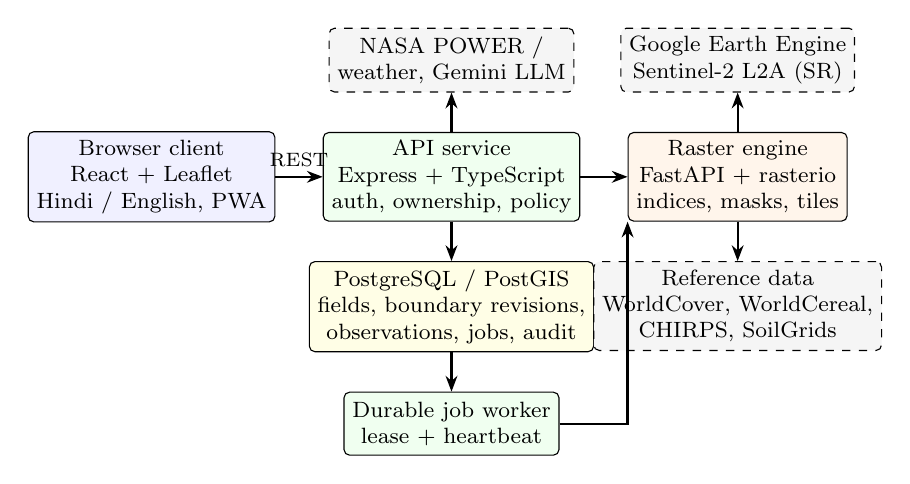
\begin{tikzpicture}[
  node distance=5mm and 6mm,
  box/.style={draw, rounded corners=2pt, align=center, font=\footnotesize, minimum height=8mm, inner sep=3pt, fill=white},
  ext/.style={box, dashed, fill=gray!8},
  arr/.style={-{Stealth[length=2mm]}, thick}]
  \node[box, fill=blue!6]   (ui)  {Browser client\\React + Leaflet\\Hindi / English, PWA};
  \node[box, fill=green!6, right=of ui]  (api) {API service\\Express + TypeScript\\auth, ownership, policy};
  \node[box, fill=orange!8, right=of api] (eng) {Raster engine\\FastAPI + rasterio\\indices, masks, tiles};
  \node[box, fill=yellow!10, below=of api] (db) {PostgreSQL / PostGIS\\fields, boundary revisions,\\observations, jobs, audit};
  \node[box, fill=green!6, below=of db] (wk) {Durable job worker\\lease + heartbeat};
  \node[ext, above=of eng] (gee) {Google Earth Engine\\Sentinel-2 L2A (SR)};
  \node[ext, below=of eng] (ref) {Reference data\\WorldCover, WorldCereal,\\CHIRPS, SoilGrids};
  \node[ext, above=of api] (wx) {NASA POWER /\\weather, Gemini LLM};
  \draw[arr] (ui) -- node[above, font=\scriptsize]{REST} (api);
  \draw[arr] (api) -- (eng);
  \draw[arr] (api) -- (db);
  \draw[arr] (db) -- (wk);
  \draw[arr] (wk.east) -| (eng.south west);
  \draw[arr] (eng) -- (gee);
  \draw[arr] (eng) -- (ref);
  \draw[arr] (api) -- (wx);
\end{tikzpicture}}
\caption{TerraScope architecture. Solid boxes are TerraScope components; dashed boxes are external providers. Only the API talks to the database; the raster engine is stateless.}
\label{fig:arch}
\end{figure}

Fig.~\ref{fig:arch} shows the three-tier architecture. The \textbf{client} is a React~19/Vite single-page application with Leaflet and OpenStreetMap for field drawing, boundary editing and overlay display; no map API key is needed. The interface is bilingual (Hindi/English) with a bundled Devanagari font, supports hectare/acre units, and adapts from 320\,px phones to desktops. The \textbf{API} (Express~5, TypeScript) handles accounts, per-field ownership checks, request limits, evidence policy and exports. The \textbf{raster engine} (FastAPI, rasterio, Shapely, Earth Engine Python API) is stateless: it receives a boundary and asset references and returns statistics, overlays or map tiles. State is kept in \textbf{PostgreSQL~18 with PostGIS~3.6}, managed by 18 additive migrations.

\subsection{Provenance-preserving data model}
A field has a polygon boundary and an integer \emph{boundary version}. Editing a boundary archives the old geometry, increments the version, invalidates summaries and fails any queued job created for the old version. Each observation stores the scene identifier, acquisition timestamp, source (Earth Engine or Earth Search), \texttt{calculation\_version}, valid-pixel count, valid coverage, an \texttt{accepted} flag with a quality reason, and one of five provenance classes: \texttt{measured\_imagery}, \texttt{user\_reported}, \texttt{public\_boundary}, \texttt{demo} and \texttt{legacy\_unverified}. Only accepted \texttt{measured\_imagery} on the current boundary version can influence an assessment, so legacy or synthetic values cannot be silently promoted.

\subsection{Durable processing jobs}
Image checks run as PostgreSQL-backed jobs rather than in the request cycle. A unique partial index on (\textit{field}, \textit{kind}) for active states deduplicates repeated requests. Workers claim jobs with \texttt{SELECT \dots{} FOR UPDATE SKIP LOCKED}, write a heartbeat every 20\,s under a random lease token, and a recovery pass re-queues jobs whose heartbeat is older than 6\,min until their attempt budget is exhausted. A job whose field boundary has changed is failed rather than allowed to attach results to the wrong geometry. Closing the browser therefore does not cancel processing, and a crashed worker cannot leave a job stuck.

\subsection{Reference datasets}
Six public sources can be attached per field, each stored as a boundary-versioned run with source, licence, retrieval time and coverage: ESA WorldCover 2021 (land-cover shares)~\cite{zanaga2022}, ESA WorldCereal 2021 temporary-crop maps via Earth Engine~\cite{vantricht2023}, CHIRPS~v3 daily rainfall~\cite{funk2015}, SoilGrids~2.0 surface properties with uncertainty quantiles~\cite{poggio2021}, NASA POWER daily weather~\cite{nasapower}, and permission-reviewed FAO crop-calendar rows. Raster downloads use bounded HTTP range requests on the intersecting tile only, and the system refuses a global-raster fallback. These sources are shown as historical or modeled \emph{context}; they are never used as the current crop identity or as soil-test results.

\subsection{Ground-truth collection with consent}
Farmers can record photo-backed scouting notes with a category, growth stage and severity. The API always stores them as \texttt{owner\_reported}/\texttt{unverified}, whatever the client submits. Per note, an owner may consent to a research field visit; consent events are append-only. A reviewer role, granted only by a database operator, unlocks a queue that shows consented field locations and dates but hides the farmer's photos, notes and labels to reduce anchoring bias. Reviewers submit independent labels with a field-visit attestation into a separate, append-only table. A pure TypeScript evaluator computes confusion-matrix metrics from \emph{expert-verified} records only, returns \texttt{null} rather than 0 for undefined denominators, and asserts that no field appears in both training and evaluation sets.

\subsection{Assistant and leaf-photo research tools}
An optional Gemini-based assistant receives recent field records with instructions to describe farmer reports as reports, not diagnoses. Leaf-photo classifiers (Section~\ref{sec:ml}) are isolated research endpoints that accept only signature-verified JPEG/PNG/WebP images under 5\,MB and 20\,MP, process uploads in memory, and return explicitly uncalibrated class scores.

%=====================================================================
\section{Field-Level Index Computation}\label{sec:engine}
%=====================================================================
\subsection{Reflectance handling and masking}
For a boundary polygon $P$ (WGS84), the engine reprojects $P$ into the CRS of the red band and builds a reference grid $G$ that covers the entire bounding box of $P$, even where it extends beyond the scene footprint. Every band is warped onto $G$ (bilinear for reflectance, nearest-neighbour for the categorical SCL) and converted to surface reflectance $\rho = s\cdot DN + o$ using the STAC \texttt{raster:bands} scale $s$ and offset $o$. If an integer band arrives without trustworthy scale and offset metadata, the engine raises an error rather than guessing. A pixel $p$ is \emph{valid} if
\begin{equation}
p \in P,\quad \mathrm{SCL}(p) \notin \mathcal{I},\quad \rho_{\mathrm{red}},\rho_{\mathrm{NIR}} \ge 0,\quad |\rho_{\mathrm{NIR}}+\rho_{\mathrm{red}}| > 10^{-12},
\end{equation}
where $\mathcal{I}=\{0,1,2,3,8,9,10,11\}$ excludes no-data, saturated/defective, dark-area, cloud-shadow, medium- and high-probability cloud, thin-cirrus and snow pixels~\cite{mainknorn2017}. A missing SCL band is an error, not a reason to skip masking.

\subsection{Indices}
Over the valid set $V$ the engine reports
\begin{align}
\NDVI &= \frac{\rho_{\mathrm{NIR}}-\rho_{\mathrm{red}}}{\rho_{\mathrm{NIR}}+\rho_{\mathrm{red}}}, \quad
\mathrm{NDRE} = \frac{\rho_{\mathrm{NIR}}-\rho_{\mathrm{RE1}}}{\rho_{\mathrm{NIR}}+\rho_{\mathrm{RE1}}},\\
\mathrm{NDMI} &= \frac{\rho_{\mathrm{NIR}}-\rho_{\mathrm{SWIR1}}}{\rho_{\mathrm{NIR}}+\rho_{\mathrm{SWIR1}}}, \quad
\mathrm{SAVI} = \frac{1.5(\rho_{\mathrm{NIR}}-\rho_{\mathrm{red}})}{\rho_{\mathrm{NIR}}+\rho_{\mathrm{red}}+0.5},\\
\mathrm{EVI} &= \frac{2.5(\rho_{\mathrm{NIR}}-\rho_{\mathrm{red}})}{\rho_{\mathrm{NIR}}+6\rho_{\mathrm{red}}-7.5\rho_{\mathrm{blue}}+1},
\end{align}
together with the mean, median, minimum, maximum and standard deviation of NDVI. Sentinel-2 bands B4, B8, B5, B11 and B2 supply red, NIR, RE1, SWIR1 and blue respectively.

\subsection{Coverage and acceptance}
The quality denominator is the number of grid cells inside the \emph{whole} boundary, so a field half outside a scene cannot appear fully observed:
\begin{equation}
C = 100\cdot\frac{|V|}{|\{p\in G : p\in P\}|}.
\end{equation}
An observation is accepted if $C \ge C_{\min}$ and $|V|\ge N_{\min}$, with defaults $C_{\min}=70\%$ and $N_{\min}=10$. Candidate scenes from the last 90 days (in the Earth Engine path, pre-filtered to \texttt{CLOUDY\_PIXEL\_PERCENTAGE}~$<40$) are processed newest first, up to six attempts. If no candidate is accepted, the previous evidence stays in place; it is not overwritten with a poorer measurement.

\subsection{Within-scene anomaly zones}
To guide scouting, pixels with $\NDVI(p) < \mu_V - 1.5\,\sigma_V$ are vectorized into ``inspection zones'' and reported as an affected-area percentage. These zones are a visit aid, not a stress classification; Section~\ref{sec:results} quantifies their behaviour.

%=====================================================================
\section{Evidence-First Assessment}\label{sec:evidence}
%=====================================================================
\begin{algorithm}[t]
\caption{Field assessment from accepted evidence}
\label{alg:assess}
\begin{algorithmic}[1]
\Require latest observation $L$, previous observation $R$, policy $(C_{\min},N_{\min},F,\delta)$
\If{$L$ is none} \Return \textsc{AwaitingAnalysis} \EndIf
\State $a \gets$ age of $L$ in days
\If{$\neg L.\mathit{accepted}$ \textbf{or} $L.\mathit{prov}\neq$ measured \textbf{or} $C_L<C_{\min}$ \textbf{or} $N_L<N_{\min}$}
  \State \Return \textsc{NotEnoughData}
\EndIf
\State $\Delta \gets$ none
\If{$R$ accepted, measured, same boundary and calculation version, earlier date}
  \State $\Delta \gets \NDVI_L - \NDVI_R$
\EndIf
\If{$a > F$} \Return \textsc{ImageTooOld} \EndIf
\If{$\Delta \neq$ none \textbf{and} $\Delta \le -\delta$} \Return \textsc{NeedsInspection} \EndIf
\If{$\Delta =$ none} \Return \textsc{NotEnoughData} \EndIf
\State \Return \textsc{NoUnusualChange}
\end{algorithmic}
\end{algorithm}

Algorithm~\ref{alg:assess} gives the assessment rule, with defaults freshness $F=14$\,days and decline threshold $\delta=0.10$. Three properties matter. First, \emph{staleness takes priority over change}: an old image yields ``image too old; current crop condition is unknown'' even if it showed no decline. Second, a single usable image never produces a reassuring state, because change requires a comparable earlier image on the same boundary version and calculation version. Third, ``no unusual change'' is worded as ``this does not rule out crop problems'', and ``needs inspection'' lists harvest, maturity and bare soil as alternative explanations. Every state maps to one next action (find a newer image, plan a field visit, continue monitoring), which the bilingual dashboard shows first.

Multi-date trends are described with an ordinary least-squares slope over \emph{elapsed days}, not observation index. Same-day duplicates are averaged so that adjacent tiles do not count twice, and at least two distinct dates are required. The engine does not predict crop stage or future NDVI. An experimental 0--100 vegetation score ($0.75$ greenness $+\,0.25$ moisture) is shown only under advanced details and never affects acceptance.

%=====================================================================
\section{Experimental Methodology}\label{sec:method}
%=====================================================================
Because no independently verified field-health labels exist yet for the deployment region, we do not report agronomic accuracy for TerraScope's assessments. Instead we evaluate (i) whether the engine measures what it claims under controlled conditions, (ii) how the default decision rules behave, and (iii) how public benchmarks behave under leakage-aware protocols.

\subsection{E1: Measurement accuracy and the coverage gate}
We drive the production \texttt{/calculate-indices} endpoint of the FastAPI engine (the same code path used for STAC assets) with synthetic GeoTIFFs on a $120\times120$ grid of $10^{-4}$\,degree ($\approx$11\,m) pixels. A square field covers 10\,000 pixels. Red reflectance is fixed at 0.08 and NIR is set so that per-pixel NDVI follows $\mathcal{N}(0.62, 0.06^2)$ exactly. Spatially clustered clouds, made by thresholding box-filtered Gaussian noise, are written into the SCL band (class~9) to cover 0--100\% of the field in steps of 5\%, with 10 random repetitions per level (210 runs). We record valid coverage, acceptance under the default policy, and absolute error against the true mean of clear pixels and of the whole field.

\subsection{E2: Sensitivity of the change rules}
For two dates, a base NDVI field $\mathcal{N}(0.70,0.05^2)$ is perturbed by independent noise $\mathcal{N}(0,0.02^2)$; on the second date a randomly placed square patch covering $f\in[0,0.6]$ of the field is reduced by 0.30 NDVI, a strong localized stress. Each of 13 levels is repeated 10 times (130 scene pairs, 260 endpoint calls). We measure the field-mean change $\Delta$, the share of pairs flagged by Algorithm~\ref{alg:assess} ($\Delta\le-0.10$), and the affected area returned by the $1.5\sigma$ zone rule.

\subsection{E3: Leakage-controlled learning baselines}\label{sec:ml}
\textit{CropHarvest crop/non-crop.} From 87\,464 checksum-verified CropHarvest~v14 samples~\cite{tseng2021} (216 features), 3\,143 duplicate-feature samples are removed. Four entire source datasets (\texttt{china-crop}, \texttt{kenya}, \texttt{lem-brazil}, \texttt{togo-eval}) are held out for testing, giving 79\,220 training and 5\,101 test samples. Cross-split location/date overlap is excluded, and no tuning uses the test set. A class-balanced random forest (100 trees, depth 12, seed 42) is trained.

\textit{Maize leaf disease.} A MobileNetV2~\cite{sandler2018} with a frozen ImageNet-pretrained backbone and a new four-class head (gray leaf spot, common rust, northern leaf blight, healthy) is trained on PlantVillage maize images~\cite{hughes2015} for 5 epochs (Adam, learning rate $10^{-3}$, batch 16, 224\,px, horizontal-flip augmentation). The split is 2\,599 training and 459 validation images, and evaluation uses the 794-image official test split.

\textit{Tabular crop-health baseline.} A previously committed baseline on a 212\,019-row tabular dataset (14 agronomic, weather and soil features, binary label) is audited against the majority-class rate.

\textit{Field-photo potato dataset.} The PLDD-UP dataset~\cite{plddup2026} (15\,519 field photographs from Uttar Pradesh: 4\,600 healthy, 4\,803 early blight, 6\,116 late blight) is inventoried with SHA-256 exact-duplicate and 64-bit difference-hash near-duplicate grouping, and groups are kept within one split. No trained-model result is reported for it, because training had not completed at the time of writing.

\subsection{E4: Live acquisition case and software verification}
We report a live public-boundary verification run and repository test results. All experiment scripts and raw outputs are in the project repository under \texttt{docs/paper/experiments}.

%=====================================================================
\section{Results}\label{sec:results}
%=====================================================================
\subsection{E1: The engine measures what it reports}
\begin{figure}[t]
\centering
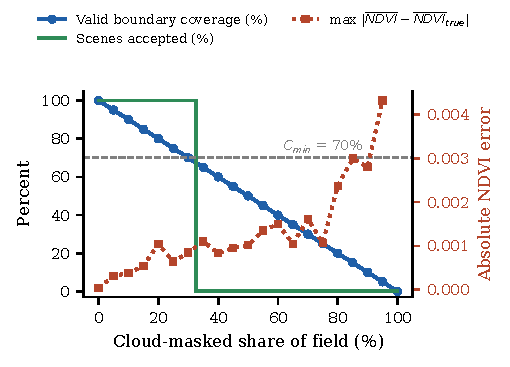
\includegraphics[width=\columnwidth]{fig_cloud_sweep.pdf}
\caption{E1: Cloud-fraction sweep through the production raster endpoint (10 runs per level). Coverage falls linearly with masked area, acceptance switches off exactly when coverage drops below $C_{\min}$, and the error of the clear-sky mean against the whole-field mean stays below 0.005 NDVI.}
\label{fig:cloud}
\end{figure}

Across all 200 runs with any clear pixel, the reported field-mean NDVI matched the true mean of clear pixels to within $5\times10^{-5}$, which is consistent with float32 rounding (Fig.~\ref{fig:cloud}). Reported coverage equalled the clear share of the boundary in every run. Acceptance was 100\% for cloud fractions up to 30\% and 0\% from 35\% upwards, so the gate behaves as specified. A fully clouded field returned HTTP~422 (``no valid pixels after masking'') instead of a number. Because clouds in E1 are independent of NDVI, the clear-sky mean differed from the whole-field mean by at most 0.0043 even at 95\% cloud. With real clouds this difference is not guaranteed, which is the reason for the coverage gate.

\subsection{E2: Default change rules are coarse}
\begin{figure}[t]
\centering
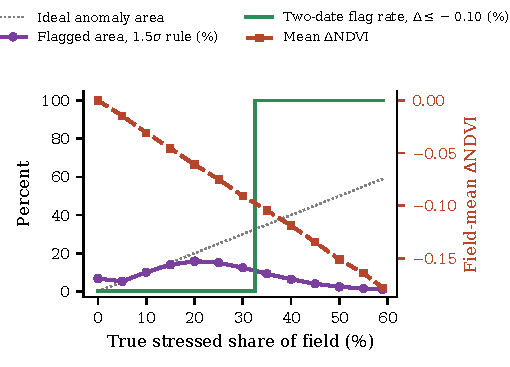
\includegraphics[width=\columnwidth]{fig_patch_sweep.pdf}
\caption{E2: Response of the two decision rules to a localized NDVI drop of 0.30 covering a growing share of the field (10 scene pairs per level). The field-mean rule flags only once about one third of the field is affected; the $1.5\sigma$ zone rule has a 6.8\% false area at zero stress and under-reports large patches.}
\label{fig:patch}
\end{figure}

\begin{table}[t]
\caption{E2: Two-date response to a localized NDVI drop of 0.30}
\label{tab:patch}
\centering
\begin{tabular}{@{}rrrr@{}}
\toprule
Stressed share & Mean $\Delta\NDVI$ & Flagged pairs & $1.5\sigma$ zone area \\
\midrule
0\%  & $-0.000$ & 0\%   & 6.8\% \\
10\% & $-0.031$ & 0\%   & 10.1\% \\
20\% & $-0.061$ & 0\%   & 15.9\% \\
30\% & $-0.091$ & 0\%   & 12.4\% \\
35\% & $-0.105$ & 100\% & 9.2\% \\
50\% & $-0.151$ & 100\% & 2.4\% \\
59\% & $-0.178$ & 100\% & 1.0\% \\
\bottomrule
\end{tabular}
\end{table}

Table~\ref{tab:patch} and Fig.~\ref{fig:patch} show that the field-mean change scales as $\Delta\approx-0.30f$, so the default threshold $\delta=0.10$ is crossed only at $f\approx 33\%$. A severe stress on a quarter of the field therefore produces ``no unusual change''. This is consistent with the conservative wording of that state, but it shows that the field-mean rule is a coarse screen. The $1.5\sigma$ zone rule has the opposite weakness. On an unstressed Gaussian field it marks 6.75\% of the area, which matches the theoretical tail mass $\Phi(-1.5)=6.68\%$. Because $\mu_V$ and $\sigma_V$ are re-estimated from the stressed scene itself, the marked area peaks at about 16\% for a 20\% patch and then falls to 1\% as the patch grows, since a widespread drop becomes the new norm. Both rules are therefore unsuitable as stress detectors without calibration. A rule that compares each pixel with its \emph{own} history on the same boundary would avoid both failure modes; we leave this for future work.

\subsection{E3: Leakage-controlled baselines}
\begin{table}[t]
\caption{E3: Learning baselines under the stated protocols}
\label{tab:ml}
\centering
\resizebox{\columnwidth}{!}{%
\begin{tabular}{@{}lccc@{}}
\toprule
Metric & \multicolumn{1}{c}{CropHarvest RF} & \multicolumn{1}{c}{Maize MobileNetV2} & \multicolumn{1}{c}{Tabular RF} \\
 & (source held out) & (official test) & (as committed) \\
\midrule
Test samples      & 5\,101 & 794 & --- \\
Accuracy          & 0.752  & 0.953 & 0.699 \\
Balanced acc.     & 0.753  & 0.939$^\dagger$ & --- \\
Precision         & 0.720  & 0.936$^\ddagger$ & --- \\
Recall            & 0.813  & 0.939$^\ddagger$ & --- \\
F1                & 0.764  & 0.937$^\ddagger$ & --- \\
ROC-AUC           & 0.793  & --- & --- \\
Majority baseline & 0.506  & 0.315 & 0.699 \\
\bottomrule
\multicolumn{4}{@{}l}{\footnotesize $^\dagger$Mean per-class recall. $^\ddagger$Macro average over four classes.}
\end{tabular}}
\end{table}

\begin{table}[t]
\caption{Maize MobileNetV2 confusion matrix on the official test split}
\label{tab:maize}
\centering
\begin{tabular}{@{}lrrrrr@{}}
\toprule
True $\backslash$ Pred. & GLS & Rust & NLB & Healthy & F1 \\
\midrule
Gray leaf spot (GLS)  & 91 & 3   & 12  & 1   & 0.839 \\
Common rust           & 0  & 216 & 1   & 0   & 0.991 \\
N. leaf blight (NLB)  & 19 & 0   & 200 & 1   & 0.924 \\
Healthy               & 0  & 0   & 0   & 250 & 0.996 \\
\bottomrule
\end{tabular}
\end{table}

Table~\ref{tab:ml} summarizes the baselines. On entirely unseen source datasets, the CropHarvest crop/non-crop forest reaches 0.752 accuracy and 0.793 ROC-AUC (confusion matrix: 1\,789 TN, 794 FP, 472 FN, 2\,046 TP). This is a plausible cross-region result, well below the in-distribution figures commonly reported, and it shows how much accuracy is lost under geographic shift. The maize classifier reaches 0.953 accuracy and 0.937 macro-F1 on the official PlantVillage test split, and most errors are confusions between gray leaf spot and northern leaf blight (Table~\ref{tab:maize}). In line with prior findings~\cite{mohanty2016,barbedo2018}, this laboratory-image result does not establish field-photo performance, which is why the field-photo PLDD-UP pipeline enforces near-duplicate-aware splits. Finally, the committed tabular baseline's accuracy (0.6990) equals its majority-class rate ($148\,198/212\,019=0.6990$), and its feature importances are nearly uniform (0.068--0.075). The model learned no usable signal and should not be cited as a crop-health result.

\subsection{E4: Live acquisition and software verification}
In a live run on a public-demonstration parcel (18~October~2026), two Sentinel-2 scenes from 3 and 5~October were accepted with 125 valid pixels and 100\% coverage (NDVI 0.3951 and 0.3355). Scenes from 17~October had only 1.38\% usable coverage and were rejected rather than averaged in. The $-0.060$ change is below $\delta$ and, because the parcel's crop identity is unverified, is reported only descriptively. Separately, an authenticated Earth Engine search of \texttt{COPERNICUS/S2\_SR\_HARMONIZED} and index calculation both succeeded, and field-level WorldCereal coverage of 99.95\% was obtained for a user field. That field's WorldCover result (78.8\% built-up, 2.5\% cropland) is inconsistent with a cropped parcel, so the interface prompts the user to verify the boundary location. This shows how reference context can expose an input problem. SoilGrids covered only 17.7\% of the same field at its 250\,m grid, and the interface states this partial coverage.

The latest repository audit records 90 passing Node/API tests (5 skipped), 10 research-metric tests, 72 Python engine tests (1 skipped) and 22 focused browser workflows. In a full browser run, 82 tests passed and 15 failed on content assertions or timeouts. We report these failures here rather than omit them. A controlled frontend benchmark rendered 20 field cards with a median of 942\,ms and a 95th percentile of 1\,042\,ms over 10 navigations. This is a rendering measurement only, not backend or provider latency. Re-running the engine suite for this paper under Python~3.9 (the project targets 3.11) gave 65 passing tests and 1 skip. One test module that needs Python~3.10 syntax and one test that needs the Google authentication package could not run.

%=====================================================================
\section{Discussion}
%=====================================================================
\textit{Honest uncertainty is a design output.} E1 shows that careful masking and a whole-boundary denominator make the reported number trustworthy as a \emph{measurement}. Whether that measurement means the crop is healthy is a separate question, and Algorithm~\ref{alg:assess} keeps the two apart. In practice, the most frequent message a farmer sees is likely to be ``image too old'' or ``not enough usable data'' during cloudy monsoon months. We consider that more useful than a stale green score.

\textit{Default thresholds are product heuristics.} E2 shows that $\delta=0.10$ trades sensitivity for few false alarms, and that within-scene $z$-score zones are self-normalizing in an unhelpful way. Both values are configurable, but calibrating them per crop and growth stage requires labelled field visits, which motivates the consent-gated reviewer workflow.

\textit{Benchmarks need provenance audits.} The tabular audit shows a common way to obtain impressive but meaningless numbers: accuracy equal to the majority-class rate. Source-held-out evaluation (CropHarvest) and official test splits (PlantVillage) give more modest but interpretable figures.

\textit{Threats to validity.} E1 and E2 use synthetic rasters with independent noise and idealized clouds; real scenes have cloud-edge effects, mixed pixels at field margins, and correlation between clouds and land cover. E2 uses a single patch shape and stress magnitude. The live case involves one public parcel with unknown crop. No user study has been conducted.

%=====================================================================
\section{Limitations and Future Work}
%=====================================================================
TerraScope does not diagnose disease, predict yield or forecast NDVI, and it has no licensed diagnosis provider. No independently verified field-health dataset with matching dates exists yet for the target region. The Telangana field-survey data identified as a candidate still needs licence, consent and field/date alignment review. Offline synchronization, a consent-aware research export and full shared-deployment hardening remain incomplete. Future work will (i) collect reviewer-verified labels to calibrate $\delta$, $C_{\min}$ and freshness per crop and season; (ii) replace within-scene $z$-scores with per-pixel temporal baselines; (iii) complete leakage-safe training and field evaluation on PLDD-UP; and (iv) run a usability study with farmers in Hindi and English.

%=====================================================================
\section{Conclusion}
%=====================================================================
We presented TerraScope, an evidence-first crop-monitoring platform that ties every Sentinel-2 measurement to its scene, boundary revision, method and provenance, and reports when the evidence is missing, old or insufficient. Controlled experiments on the production engine confirm accurate masked index computation and an exact coverage gate. They also show that simple change rules are coarse screens rather than stress detectors. Our audit of public benchmarks shows that leakage-controlled baselines give modest results. The main obstacle to credible crop-health claims is the lack of independently verified field labels rather than missing models, and TerraScope's provenance and consent infrastructure is designed to collect them.

\section*{Data and Code Availability}
The source code, migrations, experiment scripts and raw experiment outputs are available at \url{https://github.com/tusharsingh-1801/91-CHM}. Third-party datasets keep their original licences and attributions (see \texttt{datasets/ATTRIBUTION.md}).

\section*{Acknowledgment}
% TODO: acknowledge your guide, department and any funding.
The authors thank the providers of Sentinel-2 (ESA/Copernicus), Google Earth Engine, NASA POWER, CHIRPS, ISRIC SoilGrids, ESA WorldCover and WorldCereal, NASA Harvest CropHarvest, PlantVillage, and the PLDD-UP dataset authors.

\bibliographystyle{IEEEtran}
\bibliography{references}

\end{document}
